%Document setup
\documentclass[11pt, a4paper]{article}
\usepackage[a4paper, top=1in, bottom=1in, left=1in, right=1in]{geometry} %Margins

%Tables
\usepackage{multirow}
\usepackage{longtable}
\usepackage{array}
\usepackage{rotating}
\usepackage{tablefootnote}
\usepackage{makecell}
\usepackage{booktabs}

%Table commands
\newcolumntype{P}[1]{>{\centering\arraybackslash}m{#1}}

%Graphics
\usepackage{tikz}
\usetikzlibrary{matrix,chains,positioning,decorations.pathreplacing,arrows, arrows.meta,patterns,fadings,fit,backgrounds, intersections, external, shadows.blur, shapes, calc}
% ---------- Styles ----------
\tikzset{
  entity/.style={draw, rectangle, minimum width=38mm, minimum height=12mm, align=center},
  relationship/.style={draw, diamond, aspect=2.2, inner sep=1.5pt, align=center},
  attribute/.style={draw, ellipse, inner sep=1.5pt, align=center},
  derived/.style={attribute, dashed},
  note/.style={draw, rectangle, align=left, inner sep=3pt},
  link/.style={draw, -},
  total/.style={double distance=1.1pt}, % for total participation (double line)
}
\usepackage{graphicx}
\usepackage{pgfplots}
\usepackage{callouts}
\usepackage{neuralnetwork}
\usepackage{xpatch}

%Graphics commands
\pgfplotsset{compat=newest, scaled x ticks=false}
\xpatchcmd{\linklayers}{\nn@lastnode}{\lastnode}{}{}%Neural Network options
\xpatchcmd{\linklayers}{\nn@thisnode}{\thisnode}{}{}%Neural Network options
\newsavebox{\largestimage}%Box to fix subfigures
\makeatletter
\newenvironment{customlegend}[1][]{ %Adjust legends below bar charts
    \begingroup
    \let\addlegendimage=\pgfplots@addlegendimage
    \let\addlegendentry=\pgfplots@addlegendentry
    \pgfplots@init@cleared@structures
    \pgfplotsset{#1}%
}{
    \pgfplots@createlegend
    \endgroup
}
\makeatother

%Figure management
\usepackage{wrapfig}
\usepackage[export]{adjustbox}
\usepackage{float} %For the [H] option

%Figure management commands
\restylefloat{table} %For the [H] option

%Caption management
\usepackage[justification=centering]{caption}
\usepackage{subcaption}

%Caption management commands
\captionsetup[figure]{font=footnotesize}
\captionsetup[table]{font=footnotesize, singlelinecheck=off} 

%Hyperlink management
\usepackage{color}
\usepackage[hidelinks]{hyperref}

%Hyperlink management commands
\hypersetup{
  colorlinks=false,
  linktoc=all,
  linkcolor=black,
  citecolor=black,
}

%Miscellaneous non-text related 
\usepackage{pdflscape} %To convert certain pages to landscape mode. Pdf Lscape over lscape to be able to completely make a page landscape in the pdf file within itself.

%Miscellaneous text related
% Keep minted; build must use a jobname without spaces.
\ifnum\pdfshellescape=1\relax
  \usepackage{minted}
\else
  \PackageError{report}{The minted package requires -shell-escape}{Compile with -shell-escape enabled.}
\fi
\usepackage{censor} %For redactions
\usepackage{parskip}
\usepackage{setspace} %For setting spacing between
\usepackage[normalem]{ulem} %Underlining
% \usepackage{fancyhdr} %Nicer headers
% \pagestyle{fancy} %Nicer headers
\usepackage{amsmath, amsfonts, mathtools, amsthm, amssymb} %Math stuff
\usepackage{textcomp} %Not sure what this is for
\usepackage{ragged2e} %For non-justified text
\usepackage{gensymb} %Symbols such as celsius
\usepackage{titlesec} %Section formatting
\usepackage{enumitem} %Enumerate and itemize
\usepackage{titling} %Subtitle to main title of document with extra option below
\usepackage{standalone} %Include standalone tikz diagrams
\usepackage{soul}
\usepackage{cprotect} %% Protect key things from C

%Additional packages
\usepackage{physics}
\usepackage{mathdots}
\usepackage{yhmath}
\usepackage{cancel}
\usepackage{siunitx}
\usepackage{tabularx}
\usepackage{extarrows}
\usepackage[final]{microtype}

%Miscellaneous text related commands
\urlstyle{same}
% \setcounter{biburllcpenalty}{7000}
% \setcounter{biburlucpenalty}{8000}
\usemintedstyle{friendly} %Set style of source code inputs
\useunder{\uline}{\ul}{} %Underlining
\edef\svtheparindent{\the\parindent}
\newcommand{\subtitle}[1]{ %Adds subtitle to main title
  \posttitle{
    \par\end{center}
    \begin{center}\normalsize#1\end{center}
    \vskip2mm}
}
\makeatletter %Stops TOC from appearing twice in the header for fancyhdr
\renewcommand\tableofcontents{%
    \newpage
\section*{\contentsname
        \@mkboth{
%          \MakeUppercase\contentsname}{\MakeUppercase\contentsname}}
           \MakeUppercase\contentsname}{}}
    \@starttoc{toc}%
    } 
\makeatother

%Document setup
\title{Coursework - NLP research lifecycle}
\author{
    Adithya Narayanan Balaji\\
    \texttt{anb122@ic.ac.uk}\\
    \small{CID: 02300564} \\
}
\subtitle{COMP60035 Natural Language Processing}
\date{
    \vspace{10mm}
    \textbf{GitHub repository link:} \href{https://github.com/adithya-n05/NLP-PCL-Coursework-2026}{\textcolor{blue}{\texttt{https://github.com/adithya-n05/NLP-PCL-Coursework-2026}}}\\
    \textbf{Name for leaderboard:} \texttt{CactusJack}\\
    \textit{18 February 2026}
}

\begin{document}
\begin{titlepage}
  \maketitle
  \thispagestyle{empty}
\end{titlepage}
\setcounter{page}{1}
\newpage
\clearpage
\tableofcontents
\setcounter{page}{1}
\newpage
\section{Critical Paper Review (6 marks):}
\subsection{State the primary contributions of this work (2 marks):}
This paper makes four core contributions to NLP research on Patronizing and Condescending Language (PCL):

\begin{enumerate}
  \item \textbf{A new expert-annotated PCL dataset in the news domain.} The authors release \textit{Don't Patronize Me!}: 10,637 paragraphs from the News on Web corpus (2010--2018), covering 20 countries and 10 keywords (disabled, homeless, hopeless, immigrant, in need, migrant, poor families, refugee, vulnerable, women). Under their binary mapping of the original 5-point labels, 2/3/4 are treated as \textit{positive} (contains PCL) and 0/1 as \textit{negative} (No PCL), yielding 995 positive PCL examples.

  \item \textbf{A two level granularity annotation framework.} The paper contributes paragraph-level and span-level supervision. At paragraph level, it uses a graded 0--4 label derived from two annotators, with third-annotator adjudication for strong disagreements; at span level, it labels PCL spans by category (3,554 spans). This supports both binary detection and finer-grained learning.

  \item \textbf{A two-level taxonomy of PCL mechanisms.} The taxonomy has three higher-level groups with seven categories: \textbf{The Saviour} (Unbalanced power relations, Shallow solution), \textbf{The Expert} (Presupposition, Authority voice), and \textbf{The Poet} (Metaphor, Compassion, The poorer, the merrier). An ``Other'' label is defined but not used in released annotations.

  \item \textbf{Benchmarking and analysis for two tasks.} The paper defines Task 1 (binary PCL detection) and Task 2 (multi-label category prediction), and benchmarks Random, SVM-BoW, SVM-WV, BiLSTM, BERT-base/large, DistilBERT, and RoBERTa. Transformer models are strongest overall (with RoBERTa best on Task 1), and error analysis highlights why PCL remains difficult: subtle wording, subjectivity, and world-knowledge demands.
\end{enumerate}

\subsection{Identify the technical strengths that justify the paper's publication (2 marks):}
\begin{enumerate}
  \item \textbf{Annotation soundness and reliability (most important).} The paper uses a two-stage expert annotation pipeline, explicitly handles borderline cases, resolves strong disagreements with a referee annotator, and reports inter-annotator agreement at paragraph and category levels. This is the core technical strength because all downstream modelling validity depends on label quality.

  \item \textbf{Operational task design and taxonomy alignment.} The work cleanly maps theory to implementation: a two-level taxonomy is converted into two concrete NLP tasks (binary detection and multi-label categorization). This creates a coherent problem formulation where labels, task definitions, and evaluation targets are structurally consistent.

  \item \textbf{Evaluation rigor and experimental control.} The benchmark compares classical, neural, and transformer baselines under a shared protocol, with 10-fold cross-validation, reported hyper-parameter choices, and fixed random seeds. These controls materially improve internal validity and make model comparisons more credible.

  \item \textbf{Fine-grained diagnostic analysis beyond aggregate F1.} The authors provide both per-category performance breakdowns and qualitative error analysis with concrete failure examples. This strengthens the paper technically because it explains \textit{why} models fail, not only \textit{how much} they score.

  \item \textbf{Originality of the target phenomenon.} The paper targets subtle, often well-intended condescension toward vulnerable communities, which is more weakly signalled than overt abuse/toxicity tasks. This increases both technical novelty and modelling difficulty in a meaningful way.

  \item \textbf{Community utility and extensibility (least important of the strengths listed).} The dataset + taxonomy + baselines provide a reusable benchmark foundation with clear future extension paths. While this matters for impact, it is downstream of the stronger methodological strengths above.
\end{enumerate}

\subsection{Highlight the key weaknesses or areas where the authors failed to provide sufficient evidence (2 marks):}
Ranked from biggest to smallest weakness:
\begin{enumerate}
  \item \textbf{Generalization beyond the curated dataset is not demonstrated.} Data collection is constrained to news paragraphs retrieved through ten predefined vulnerability keywords, and evaluation is only in-corpus via 10-fold cross-validation. To support a stronger claim of practical robustness, the paper needed out-of-domain testing (e.g., non-keyword retrieval, other sources such as social media/NGO text, or time-split validation).

  \item \textbf{Label uncertainty is measured but not carried into the experimental claims.} Paragraph-level agreement is moderate when borderline cases are included, yet model evaluation collapses labels into a hard binary target without uncertainty-aware analysis. The paper needed sensitivity checks showing how results change under alternative treatments of borderline/disagreement-heavy instances.

  \item \textbf{Performance differences are not backed by statistical reliability analysis.} Reported results are point estimates only, so close model gaps (especially among transformer variants) are hard to interpret as reliable improvements. The paper needed fold-level variance summaries and significance testing or confidence intervals for key pairwise comparisons.

  \item \textbf{Key modelling decisions are not isolated with ablations.} The study benchmarks multiple model families but does not decompose which design choices are responsible for gains in each task. Stronger evidence would include controlled ablations, especially testing whether using span-boundary supervision improves Task 2 over the paragraph-only framing.

  \item \textbf{Reproducibility is good but still short of a full replication recipe.} Several core settings are provided (e.g., epochs, batch size, seed), but important details remain under-specified for exact reruns across implementations. The paper needed a more complete training recipe (full optimisation schedule, selection protocol, and preprocessing details) to satisfy stricter reproducibility standards.
\end{enumerate}

\newpage
\section{Exploratory Data Analysis (EDA, 6 marks):}
\subsection{Analyse the PCL dataset using 2 distinct EDA techniques (3 marks each):}
For marking clarity, we report exactly two techniques in the required format (Visual/Tabular Evidence, Analysis, Impact Statement). We have included both a table and figure for each technique to allow for easier analysis of the EDA techniques chosen.

\subsubsection{Technique 1: Class Distribution (Binary Imbalance Audit)}
\textbf{Visual/Tabular Evidence:}
\begin{table}[H]
  \centering
  \begin{tabular}{lrrrrr}
    \toprule
    Split & Total & No\_PCL (0) & PCL (1) & PCL (\%) & No\_PCL:PCL \\
    \midrule
    Train & 8375  & 7581        & 794     & 9.48     & 9.55:1      \\
    Dev   & 2094  & 1895        & 199     & 9.50     & 9.52:1      \\
    \bottomrule
  \end{tabular}
  \caption{Binary class distribution on the official train/dev splits (derived from the provided SemEval split files).}
  \label{tab:eda_class_dist}
\end{table}

\begin{figure}[H]
  \centering
  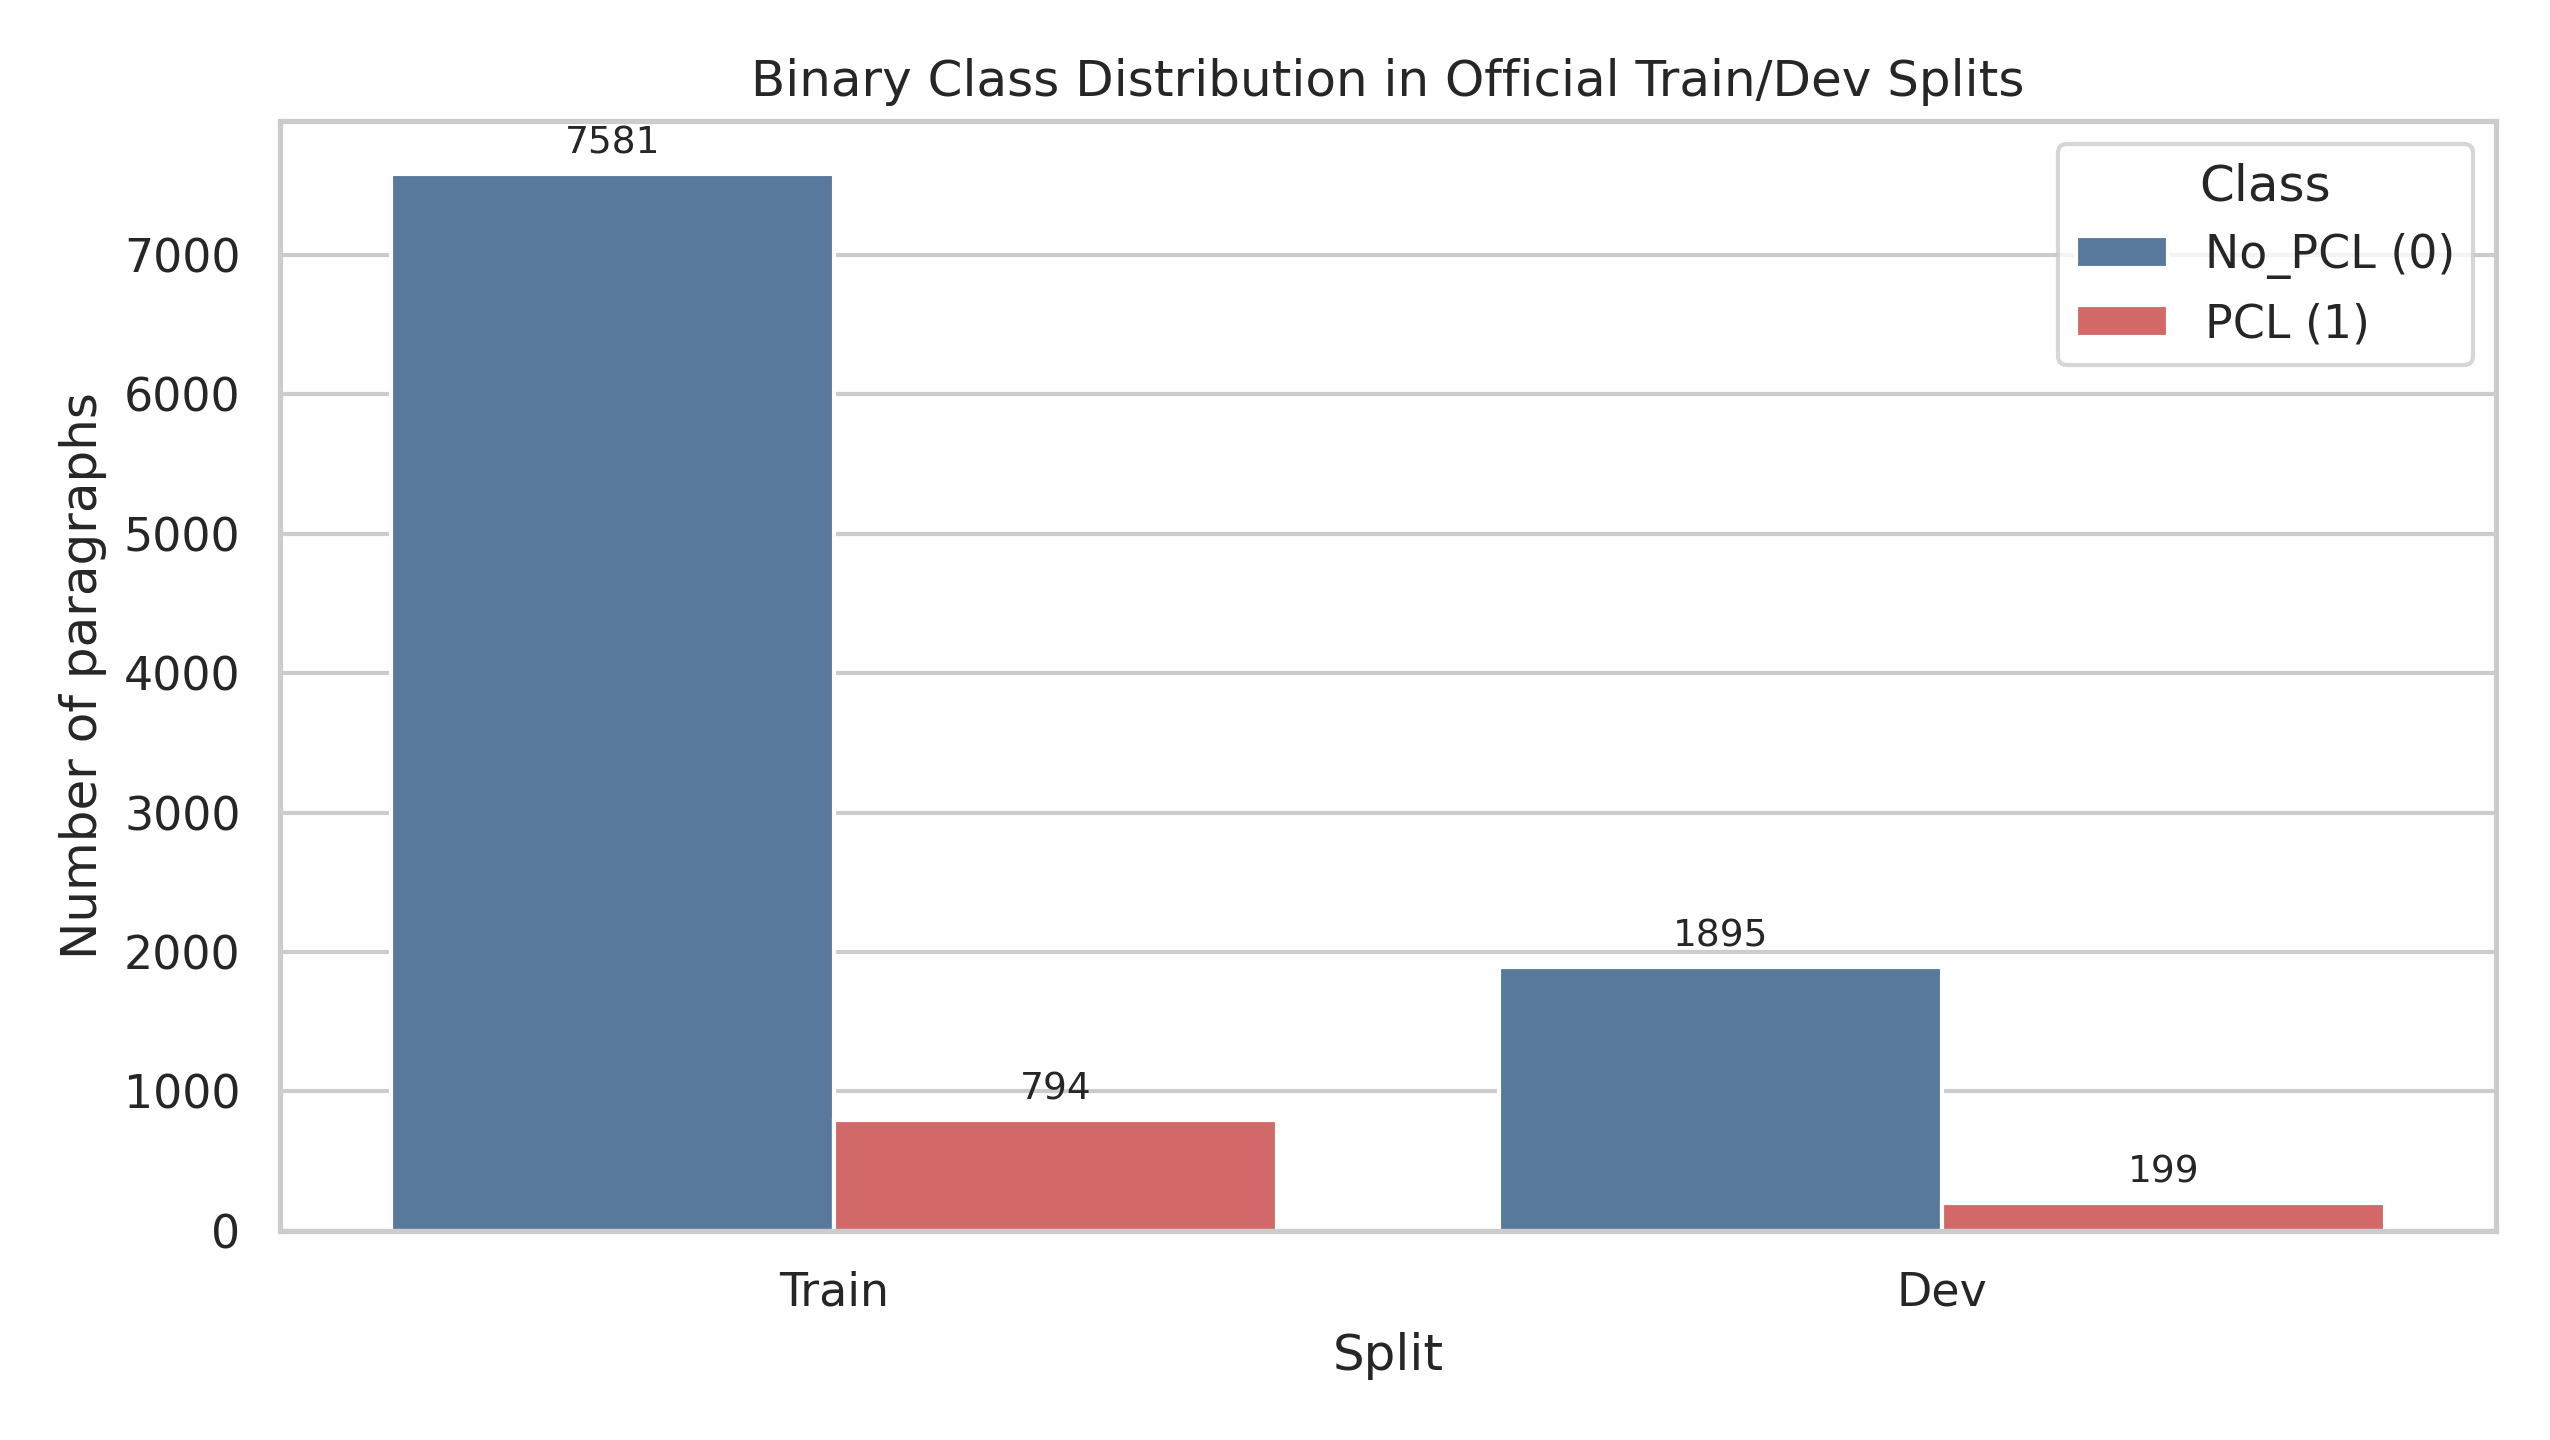
\includegraphics[width=0.85\linewidth]{figures/eda_class_distribution_train_dev.png}
  \caption{Severe and consistent class imbalance across official train/dev splits.}
  \label{fig:eda_class_dist}
\end{figure}

\textbf{Analysis:}
The dataset is highly imbalanced in both official splits: roughly 9.5\% positive (PCL) and 90.5\% negative (No\_PCL). The imbalance pattern is very consistent between train and dev, which suggests this is a true task property rather than split noise. This also means accuracy would be a misleading primary metric because a majority-class predictor would already appear strong.

\textbf{Impact Statement:}
This EDA directly informs the modelling strategy. First, model selection and reporting should prioritise positive-class F1 (as required by the spec) rather than accuracy. Second, training should explicitly handle imbalance (e.g., class-weighted loss and/or sampling) to avoid collapsing to the majority class. Third, threshold tuning on dev is required to control the precision-recall trade-off for the minority positive class. This creates a concrete route to improving over the weak baseline while remaining methodologically justified.

\subsubsection{Technique 2: Token Count and Length Outliers (Sequence Budget Audit)}
\textbf{Visual/Tabular Evidence:}

\begin{table}[H]
  \centering
  \begin{tabular}{lrrrrr}
    \toprule
    Slice              & Mean  & Median & p95   & p99    & Max \\
    \midrule
    Train (all)        & 43.53 & 38.0   & 92.0  & 128.0  & 821 \\
    Dev (all)          & 42.46 & 37.0   & 90.0  & 129.07 & 259 \\
    Train PCL only     & 47.97 & 42.0   & 103.0 & 131.0  & 458 \\
    Train No\_PCL only & 43.06 & 37.0   & 91.0  & 127.2  & 821 \\
    \bottomrule
  \end{tabular}
  \caption{Token-length statistics (word-level regex tokenisation) for official splits and train class slices.}
  \label{tab:eda_token_len}
\end{table}

\begin{figure}[H]
  \centering
  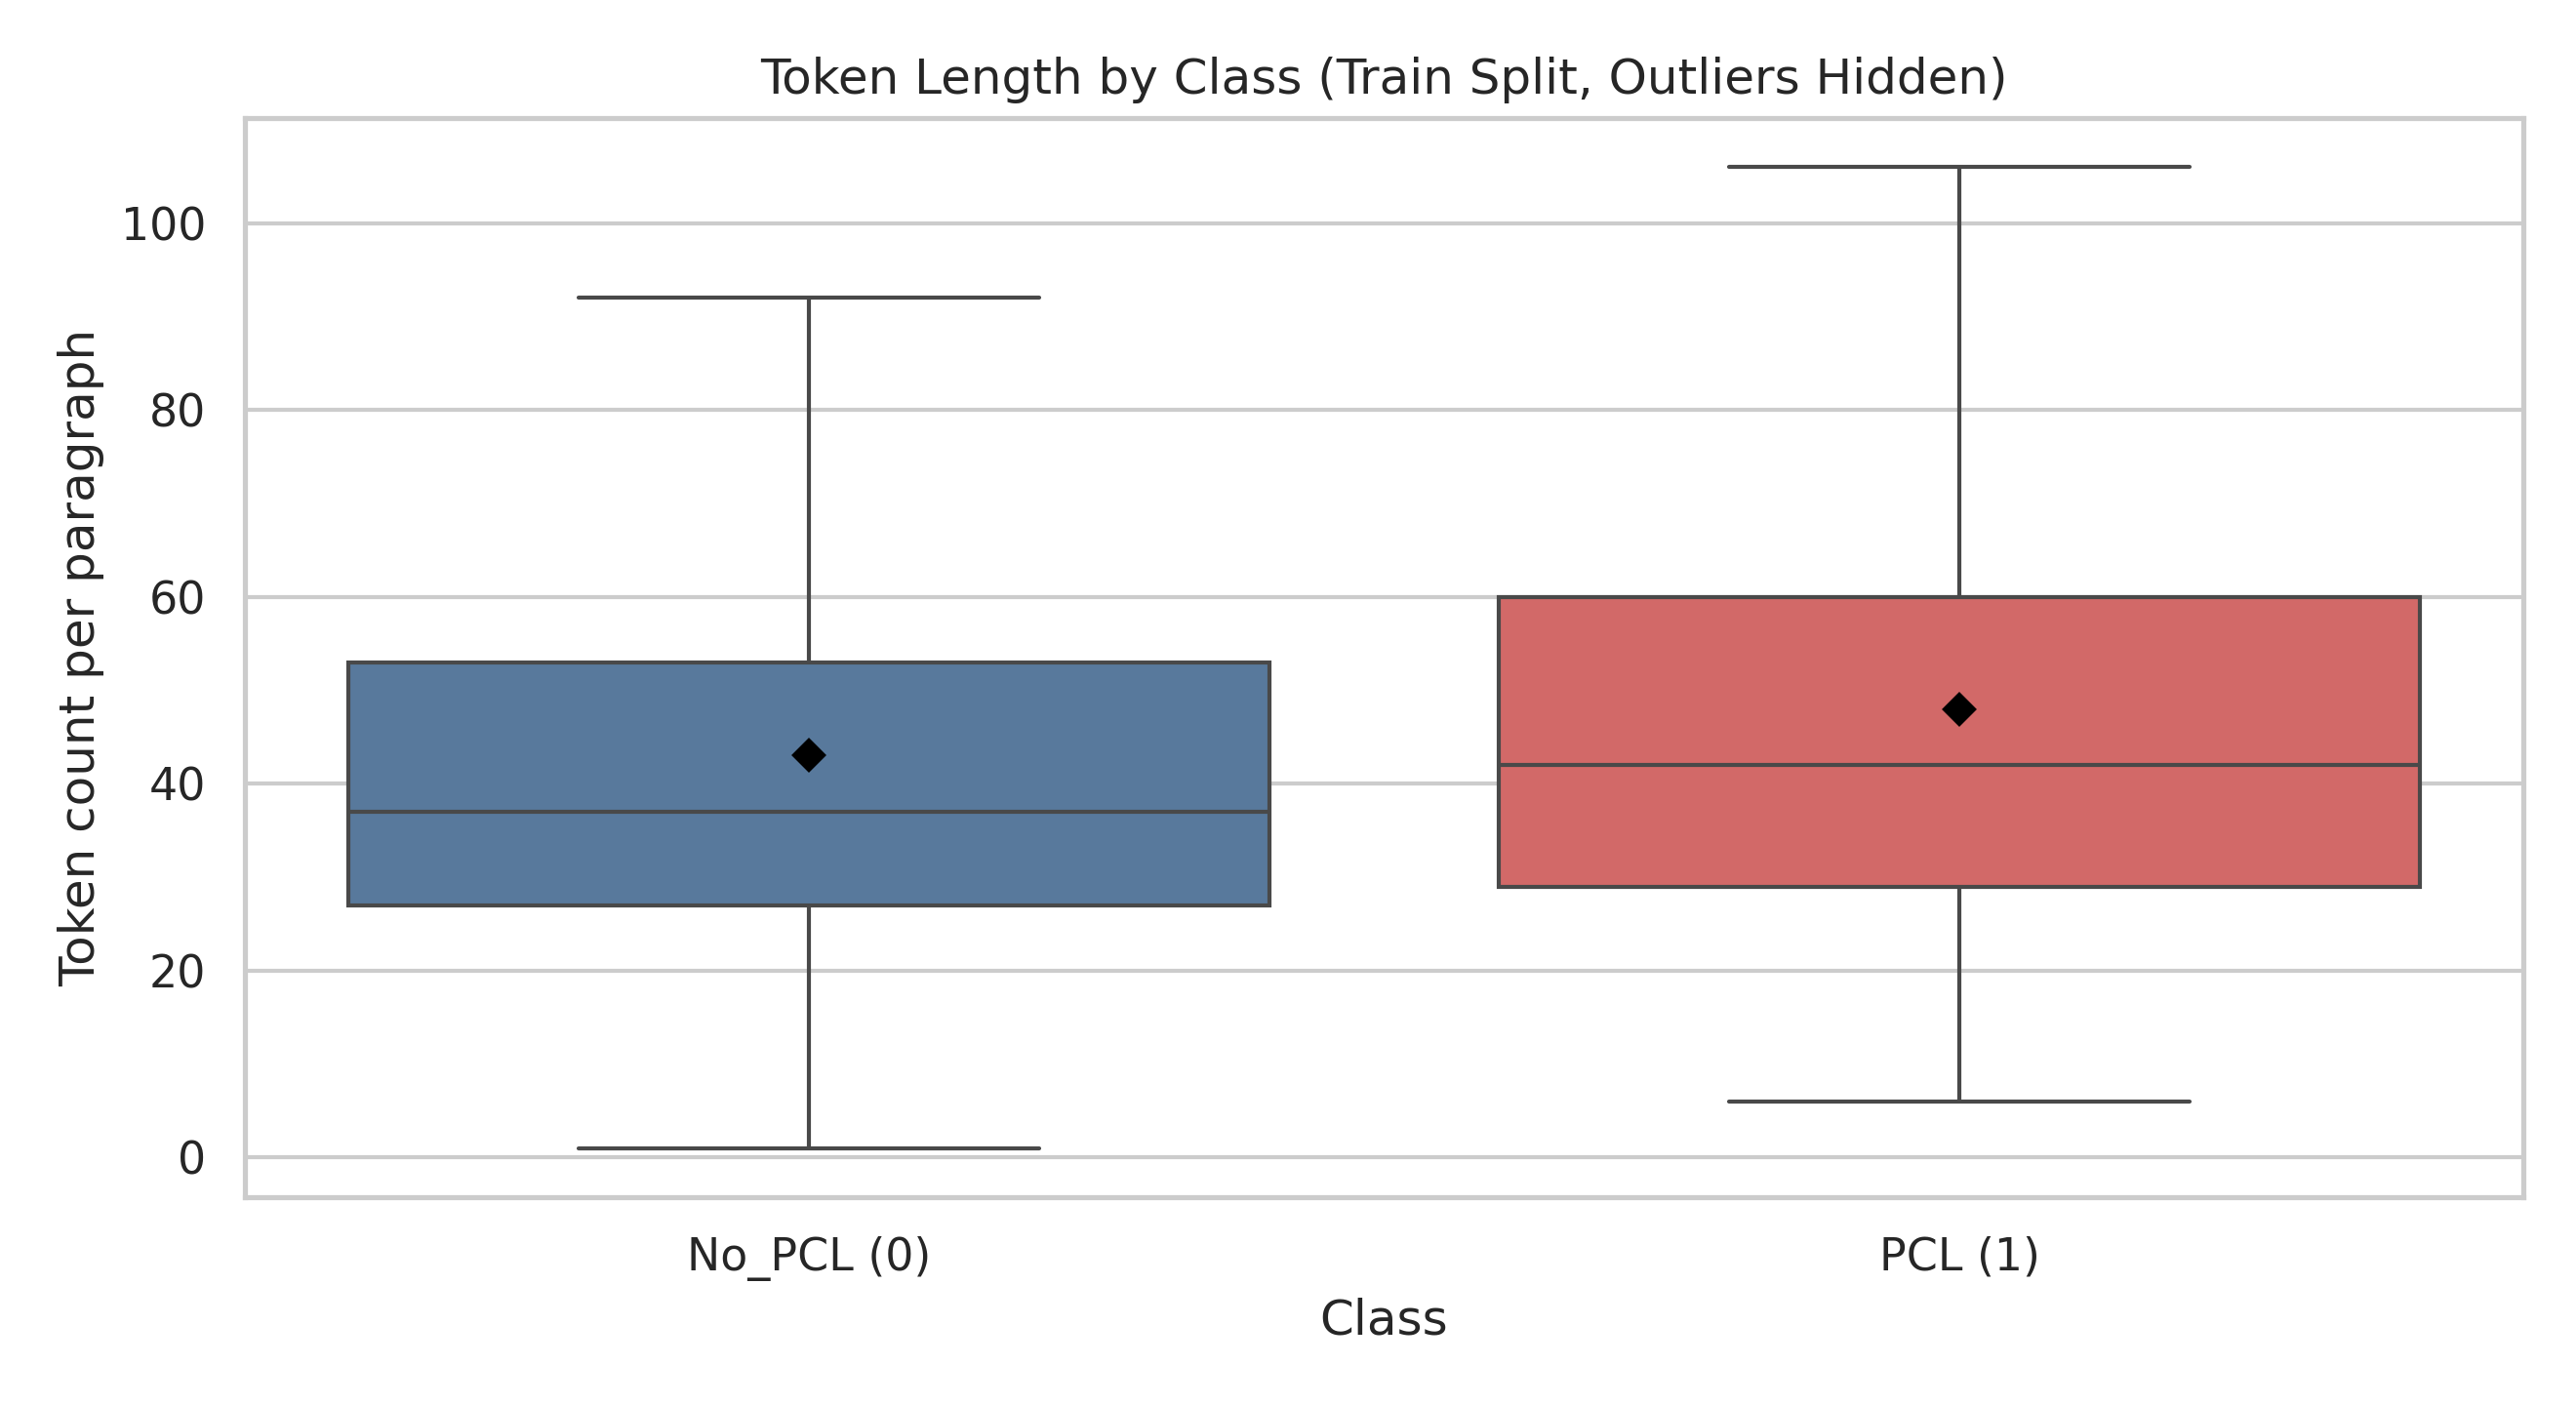
\includegraphics[width=0.85\linewidth]{figures/eda_token_length_by_class_train.png}
  \caption{Train token-length distribution by class (outliers hidden in boxplot for readability).}
  \label{fig:eda_token_len}
\end{figure}

\textbf{Analysis:}
Sequence lengths are stable across train/dev at the distribution level (means around 42--44 and medians around 37--38), so the split appears structurally consistent. However, there is a long right tail (train max 821; p99 around 128), which makes truncation a non-trivial design decision. Positives are systematically longer than negatives in train (mean 47.97 vs 43.06; p95 103 vs 91), indicating that aggressive truncation risks discarding informative positive-class context.

\textbf{Impact Statement:}
This EDA shapes both architecture settings and training protocol. We should treat \texttt{max\_length} as a tuned hyperparameter (rather than a default), selecting a value that retains most positive evidence while keeping compute feasible (e.g., around the high-percentile range with ablation checks). It also motivates outlier-aware error analysis, since very long paragraphs can drive false negatives after truncation. Together with Technique 1, this supports a novel yet defensible approach: imbalance-aware training plus calibrated decision thresholds under an explicitly justified sequence-length policy.

\newpage
\section{Describe your proposed approach (4 marks):}
Prior to model development, we first verified that the official baseline setup reproduced the expected weak baseline scores (approximately 0.48 F1 on dev and 0.49 F1 on test). We then built our final approach on top of that baseline.
\subsection{Proposed approach (2 marks):}
The core strategy is to build a multi-architecture ensemble: keep RoBERTa-base as the baseline foundation and add DeBERTa-v3-base as a complementary encoder. We chose DeBERTa-v3 because it gives a different representation style from RoBERTa on subtle linguistic cues, which helps reduce correlated errors when the two models are ensembled, whilst being of comparable performance to RoBERTa. On top of this, we improved reliability through imbalance-aware training, multi-seed training, and calibrated ensembling. We detail all key baseline changes below.

\textbf{Changes introduced over baseline:}
\begin{enumerate}
  \item \textbf{Threshold optimisation and final recalibration (F1-targeted).} In this setup, each paragraph gets a positive-class probability \(p\), and prediction is made by a one-way cutoff: predict class \(1\) if \(p \ge t\), else class \(0\). Instead of fixing \(t=0.5\), we searched \(t \in [0.05, 0.95]\) with step \(0.005\) to maximise positive-class F1. After final retraining, we repeated this threshold search on final dev probabilities so the cutoff matched the final ensemble probability scale.
  \item \textbf{Multi-architecture ensembling.} We moved from one backbone to two backbones (RoBERTa-base and DeBERTa-v3-base) so that final predictions combine complementary error profiles rather than relying on one encoder.
  \item \textbf{Multi-seed training with explicit selection and retraining.} We trained both architectures across seeds \(42, 1337, 627345\) in the scout stage, ranked all scout runs by internal-validation positive-class F1, kept the top-\(k=4\) runs, and then retrained only those selected runs on full official train for the final ensemble.
  \item \textbf{Weighted ensemble aggregation (soft voting).} ``Soft voting'' means we combine probabilities, not hard labels. For each example, if models output \(p_1,\dots,p_k\), we compute \(p_{\text{ens}}=\sum_i w_i p_i\), where \(w_i\) are normalised weights from internal-validation F1. We then apply one threshold to \(p_{\text{ens}}\). This lets stronger runs influence the final decision more than weaker runs.
  \item \textbf{Imbalance-aware sampling.} We introduced \texttt{WeightedRandomSampler} with inverse-frequency class weighting in the dataloader. Concretely, class-0 samples use weight \(1.0\), and class-1 samples use weight \(N_{\text{neg}}/N_{\text{pos}}\). The practical effect is that positive examples are sampled much more often per epoch, so gradient updates are less dominated by the majority class.
  \item \textbf{Grouped internal validation protocol.} We used grouped stratified splitting by \texttt{article\_id} (5 folds, fixed fold index 0, split seed 42) to make run selection more robust by reducing article-level leakage between train and validation.
  \item \textbf{Optimiser and schedule upgrade.} We used AdamW with learning rate \(2\times10^{-5}\), weight decay \(0.01\), \textbf{cosine annealing}, and linear warmup (\(0.1\) warmup ratio). In implementation terms, learning rate increases linearly during the first 10\% of steps (warmup), then decays smoothly with a cosine curve toward near-zero. This prevents large unstable updates at the start and makes later updates progressively finer.
  \item \textbf{Context-length and training-configuration choices.} We increased max sequence length to \(256\), used batch sizes \(16/64\), trained for 4 epochs per run, and ran in full precision (no mixed precision) for stable and consistent training behaviour across machines.
  \item \textbf{Input text cleanup before tokenization.} We applied a lightweight normalization pass before tokenization: HTML entity unescaping, removal of HTML tags, and whitespace normalization. This reduces formatting noise while preserving the underlying sentence meaning.
  \item \textbf{Scout-stage early stopping.} During scout runs only, we enabled early stopping on internal-validation positive-class F1 (patience \(=2\)). This reduces wasted training once validation improvements plateau and keeps run selection focused on generalization rather than late-epoch overfitting.
\end{enumerate}

\subsection{Rationale and Expected outcome (2 marks):}
The changes in Section 3.1 were made to address concrete weaknesses we observed in the data and in baseline behaviour.

\begin{itemize}
  \item \textbf{Why we changed class balancing:} This follows directly from EDA Technique 1 (class distribution): only about 9.5\% of examples are positive. Without correction, most gradient updates come from negative examples, so the model learns a conservative boundary and under-predicts class 1. We therefore used inverse-frequency weighted sampling so positive examples are sampled much more frequently (in practice, close to balanced exposure per epoch rather than 9.5\%), and paired this with threshold tuning so the final boundary is not stuck at an overly conservative default.

  \item \textbf{Why we changed sequence length:} This follows directly from EDA Technique 2 (token-length and outlier audit): positive examples are, on average, longer than negatives, and the dataset has a long right tail. With short truncation limits, key evidence is often cut off in exactly the cases where PCL is subtle. We increased max length to 256 to keep more of that context and reduce truncation-driven false negatives.

  \item \textbf{Why we changed seed strategy:} EDA Technique 1 implies a hard minority-class regime, where small optimisation differences can cause large swings in positive predictions. One seed and one run gave unstable outcomes. We therefore trained multiple seeds, ranked scout runs by internal-validation positive-class F1, kept the top-\(k\) runs, retrained those selected runs on full train, and then ensembled them. This turns seed variation into a selection advantage rather than a source of noise.

  \item \textbf{Why we changed model architecture:} The EDA combination (minority positives from Technique 1 + longer, subtler positive contexts from Technique 2) increases the chance that one encoder will miss certain patterns. We combined RoBERTa and DeBERTa so that one model can compensate when the other misses a case. We then used weighted soft voting so stronger runs contribute more to the final probability.

  \item \textbf{Why we changed the learning-rate schedule:} Given Technique 1 imbalance, early fine-tuning can be noisy and over-reactive to majority-class gradients. We used linear warmup followed by cosine annealing so the optimiser does not take large unstable steps at the start, then gradually shifts to finer updates later. This made training behaviour more consistent across runs.

  \item \textbf{Why we changed split/selection protocol:} This is mainly a validity control, not a change in the core approach. If related paragraphs leak across train and validation, selection looks better than it really is, and we end up choosing a brittle configuration. We used grouped internal splitting by \texttt{article\_id} to make selection estimates more trustworthy, then preserved official ordering and exact line counts for \texttt{dev.txt}/\texttt{test.txt} so evaluation remains valid. This was a minor additional change we added to ensure that the selection process was valid and that the evaluation outputs were valid.

  \item \textbf{Why we changed input text cleanup:} The dataset includes markup and formatting artefacts (for example HTML entities/tags and inconsistent spacing). If this noise is passed directly to the tokenizer, it creates avoidable token fragmentation and unstable input patterns. We therefore used minimal cleanup before tokenization so the model sees cleaner, more consistent text without altering task semantics.

  \item \textbf{Why we changed scout-stage stopping behaviour:} On this imbalanced dataset, validation F1 often peaks before the final epoch during scout runs. Continuing past that point can make selection noisy and cost unnecessary compute. Early stopping in scout runs keeps candidate selection closer to the true generalizing checkpoint while reducing tuning time.
\end{itemize}

\textbf{Expected outcome:}
\begin{itemize}
  \item \textbf{Clear improvement above the weak baseline.} Given the changes aimed at the minority-class failure modes, we would expect performance to move from baseline-level scores into the high-0.5s and potentially around the low-0.6 range on dev, with hidden-test behaviour in a similar band.
  \item \textbf{A better recall--precision balance for class 1.} With imbalance-aware sampling and threshold calibration, we would expect stronger positive recall with an acceptable precision trade-off, yielding a net gain in positive-class F1 rather than a majority-class accuracy effect.
  \item \textbf{More stable results than single-run training.} With multi-seed selection and weighted soft-vote ensembling, we would expect smaller run-to-run swings and less dependence on one lucky seed.
  \item \textbf{Fewer long-context misses.} From EDA Technique 2, we would expect a modest reduction in false negatives where key PCL cues appear later in longer paragraphs.
  \item \textbf{Valid outputs for official evaluation.} We would expect these gains while preserving Stage 5 validity constraints: train-focused model fitting, and correctly ordered/structured \texttt{dev.txt} and \texttt{test.txt}.
\end{itemize}
\newpage

\setcounter{section}{4}
\section{Evaluation and Error Analysis (11 marks):}
\subsection{Global Evaluation (6 marks):}

\textbf{Final system summary:}
Table \ref{tab:final_system_performance} is included to explain how the final score was obtained, rather than only reporting one headline number. The scout columns (\textit{Scout val F1} and \textit{Scout dev F1}) show how runs were selected on the partitioned internal-validation workflow, while the \textit{Final dev F1} column shows what happened after retraining selected runs on full official train.
\begin{table}[H]
  \centering
  \scriptsize
  \begin{tabularx}{\linewidth}{>{\raggedright\arraybackslash}X c c c c}
    \toprule
    System / Run & Scout val F1 & Scout dev F1 & Final dev F1 & Threshold \\
    \midrule
    DeBERTa-v3 (s=1337) & 0.6817 & 0.5907 & 0.6076 & 0.945 \\
    DeBERTa-v3 (s=627345) & 0.6775 & 0.5763 & 0.6146 & 0.910 \\
    DeBERTa-v3 (s=42) & 0.6426 & 0.5876 & 0.5979 & 0.935 \\
    RoBERTa-base (s=42) & 0.6343 & 0.5714 & 0.5714 & 0.665 \\
    \midrule
    Scout weighted ensemble & 0.6772 & 0.6071 & -- & 0.485 \\
    Final ensemble (pre-retune; selection threshold) & -- & -- & 0.6037 & 0.485 \\
    \textbf{Final ensemble (retuned on dev)} & -- & -- & \textbf{0.6336} & \textbf{0.250} \\
    \bottomrule
  \end{tabularx}
  \caption{Final system performance using the selected four ensemble members. Scout metrics are from grouped train-internal validation and official dev during selection; final dev metrics are measured after full-train retraining.}
  \label{tab:final_system_performance}
\end{table}
\textbf{Submission files and format checks:}
The final outputs are placed at the repository root. \texttt{dev.txt} has 2094 lines and \texttt{test.txt} has 3832 lines, with one prediction per line in official order.

\textbf{Improvement over baseline:} The final dev score is \(0.6336\) (positive-class F1). Compared with the coursework baseline of \(0.4800\), this is an absolute gain of \(+0.1536\) F1 points and a relative gain of \(+32.0\%\). This provides clear evidence that the proposed changes produced a meaningful improvement over the baseline.

\subsection{Local Evaluation (5 marks):}
\subsubsection{Error Analysis (2.5 marks):}
\textbf{Evaluation setup:}
For local error analysis, we inspected the final ensemble predictions on the official dev split (2094 examples) against the official binary Task 1 labels from \texttt{dev\_semeval\_parids-labels.csv} (1 = PCL, 0 = No PCL). This follows the coursework guidance for local evaluation and keeps analysis aligned with the official metric (positive-class F1).
\begin{figure}[H]
  \centering
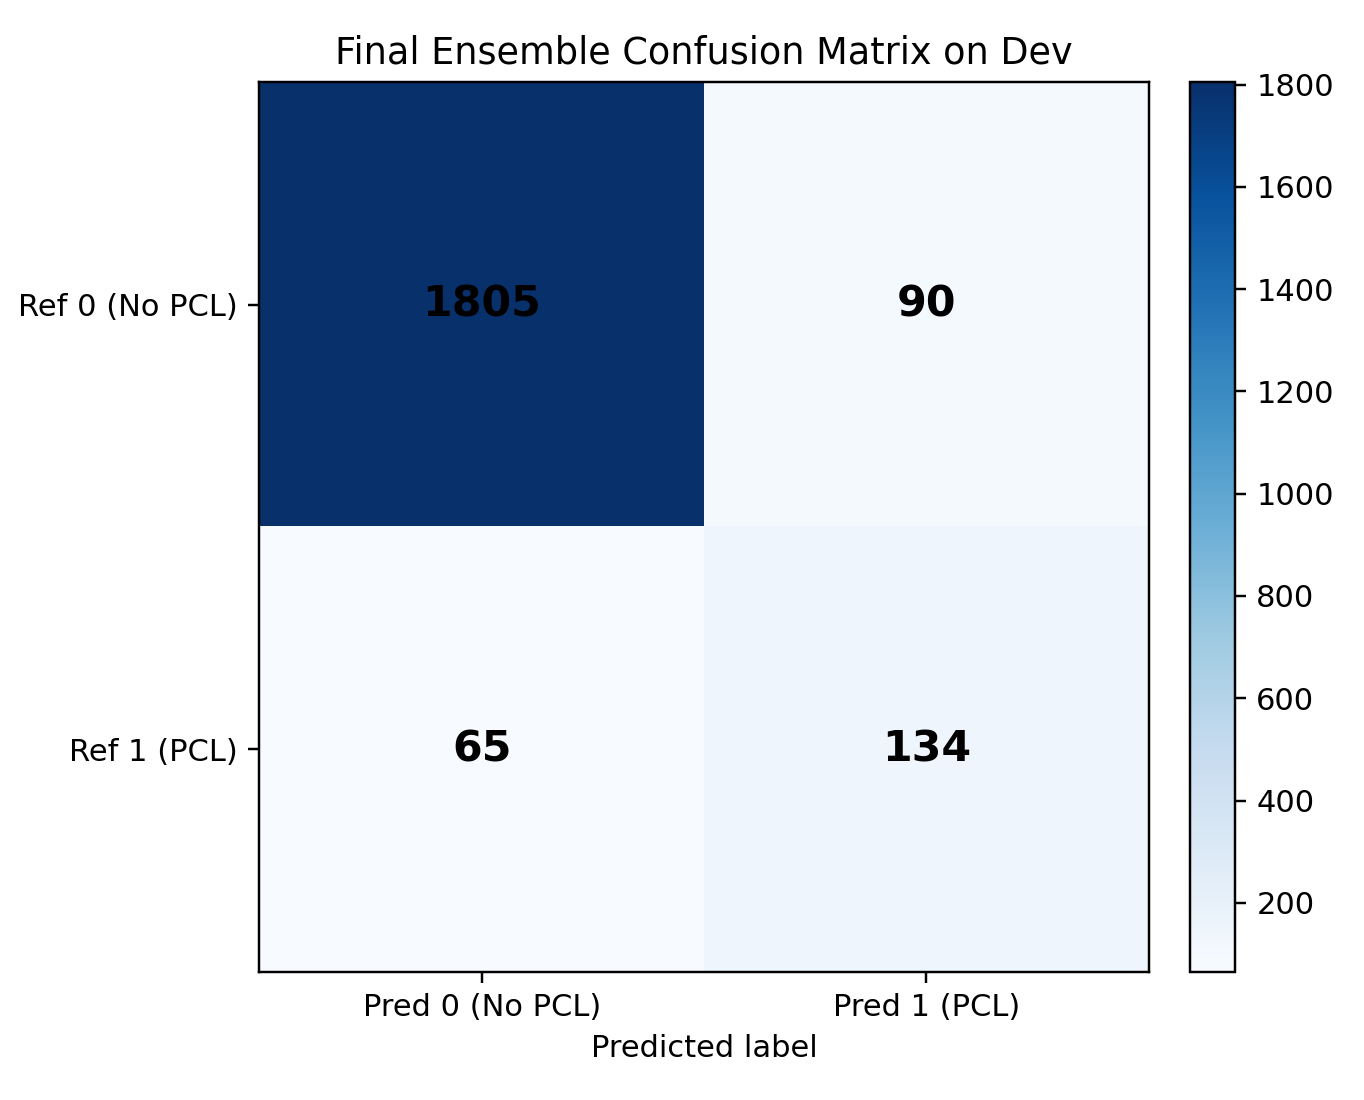
\includegraphics[width=0.4\linewidth]{figures/error_confusion_matrix_dev.png}
  \caption{Confusion matrix on official dev (evaluated against official reference labels) for the final retuned ensemble at threshold \(=0.25\).}
  \label{fig:error_confusion_dev}
\end{figure}

\textbf{Interpretation of Figure \ref{fig:error_confusion_dev}:}
The final ensemble correctly classifies \(1939/2094\) examples (\(92.60\%\) accuracy), with \(1805\) true negatives and \(134\) true positives. Although the raw false-positive count is higher (90 vs 65), the \emph{error rate} is dominated by missed positives (FNR \(32.7\%\) vs FPR \(4.75\%\)), which is why recall is improved but still not saturated.

\begin{table}[H]
  \centering
  \scriptsize
  \begin{tabularx}{\linewidth}{l c >{\raggedright\arraybackslash}X}
    \toprule
    Metric & Value & Interpretation \\
    \midrule
    Threshold & 0.2500 & Final decision cutoff used for ensemble probabilities on dev. \\
    TN & 1805 & Correctly rejected No-PCL examples (strong negative control). \\
    FP & 90 & Non-PCL examples incorrectly flagged as PCL (over-triggering). \\
    FN & 65 & PCL examples missed by the model (main residual failure mode). \\
    TP & 134 & PCL examples correctly identified. \\
    Precision (PCL) & 0.5982 & About 59.8\% of predicted positives are truly PCL. \\
    Recall (PCL) & 0.6734 & About 67.3\% of true PCL examples are recovered. \\
    F1 (PCL) & 0.6336 & Main coursework metric balancing PCL precision and recall. \\
    Accuracy & 0.9260 & High overall accuracy, but less informative under class imbalance. \\
    Specificity (TNR) & 0.9525 & Very strong true-negative rate on the majority class. \\
    False Positive Rate & 0.0475 & Roughly 4.8\% of negatives are incorrectly flagged positive. \\
    False Negative Rate & 0.3266 & Roughly 32.7\% of positives are still being missed. \\
    Negative Predictive Value & 0.9652 & Predicted negatives are very reliable in this setup. \\
    Balanced Accuracy & 0.8129 & Mean of TPR and TNR; more stable under class imbalance. \\
    AUPRC & 0.6472 & Threshold-free ranking quality for the positive class. \\
    \bottomrule
  \end{tabularx}
  \caption{Quantitative error-analysis dashboard for the final ensemble on official dev.}
  \label{tab:error_metric_dashboard_dev}
\end{table}

\textbf{Interpretation of Table \ref{tab:error_metric_dashboard_dev}:}
At the chosen threshold \(0.2500\), the model reaches precision \(0.5982\), recall \(0.6734\), and F1 \(0.6336\), with a strong negative-class profile (specificity \(0.9525\), FPR \(0.0475\), NPV \(0.9652\)). The false-negative rate is \(0.3266\), so the main remaining limitation is still under-detection of subtle PCL.

\begin{figure}[H]
  \centering
  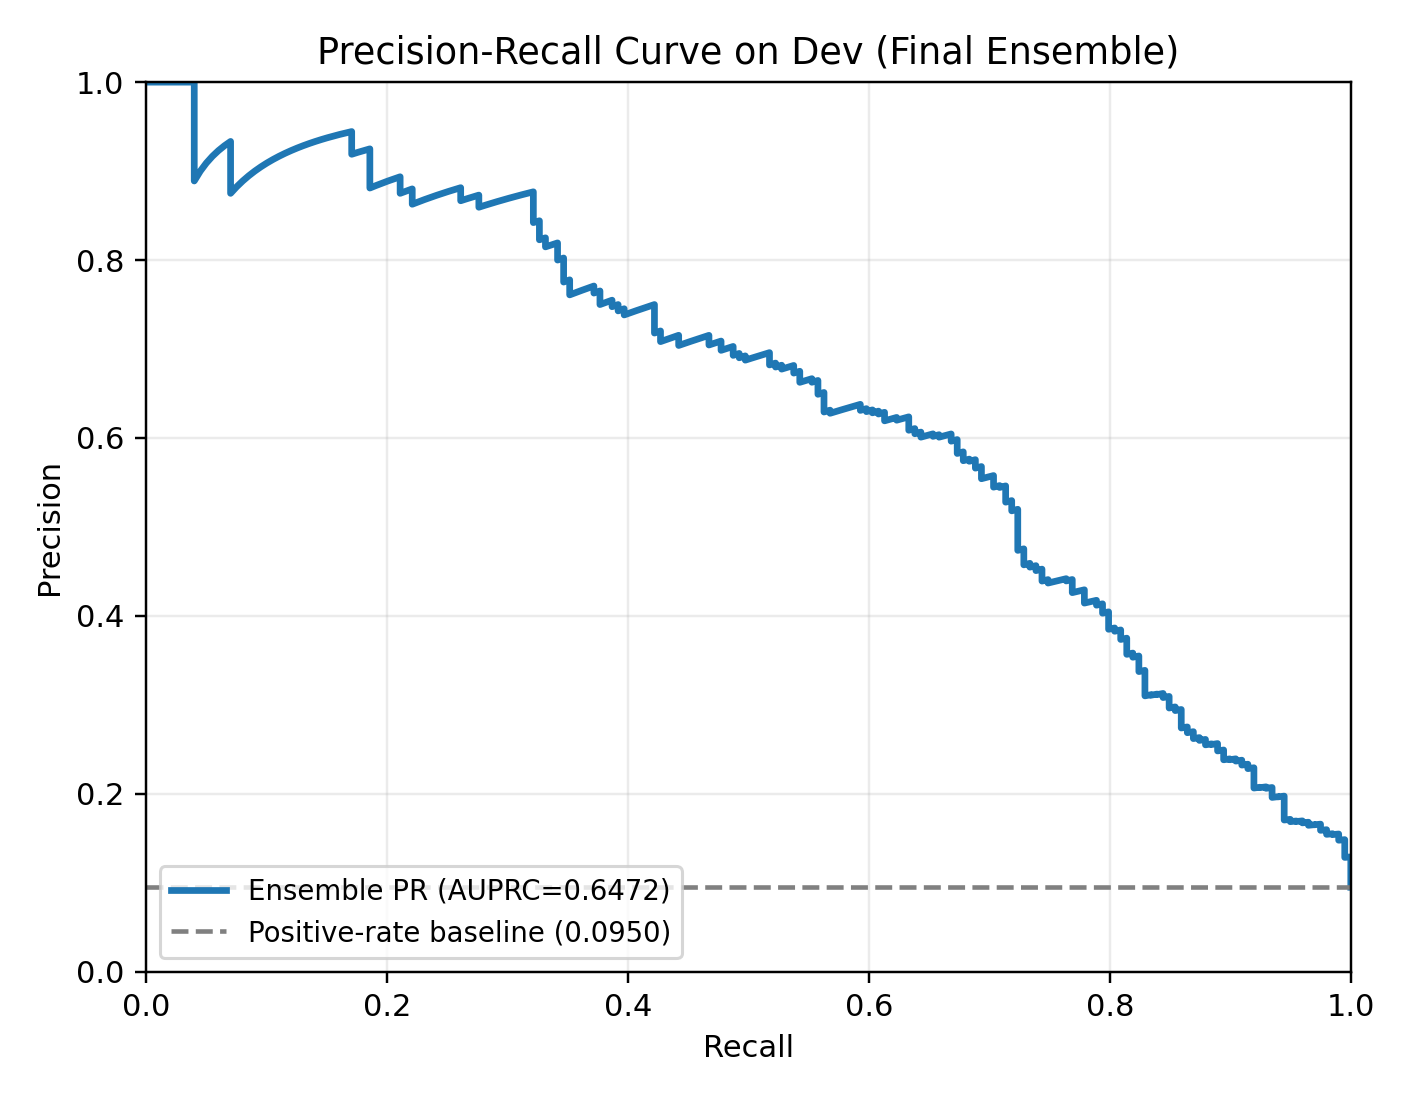
\includegraphics[width=0.66\linewidth]{figures/error_precision_recall_curve_dev.png}
  \caption{Precision-recall curve of the final ensemble on dev. The area under the PR curve is \(0.6472\), indicating stronger-than-baseline ranking of positives across thresholds.}
  \label{fig:error_pr_curve_dev}
\end{figure}

\textbf{Interpretation of Figure \ref{fig:error_pr_curve_dev}:}
The AUPRC is \(0.6472\), which supports that the ensemble probability ranking is useful beyond one fixed operating point. This aligns with the observed threshold behaviour: the retuned threshold \(0.25\) increases positive recovery while preserving acceptable precision.

\begin{figure}[H]
  \centering
  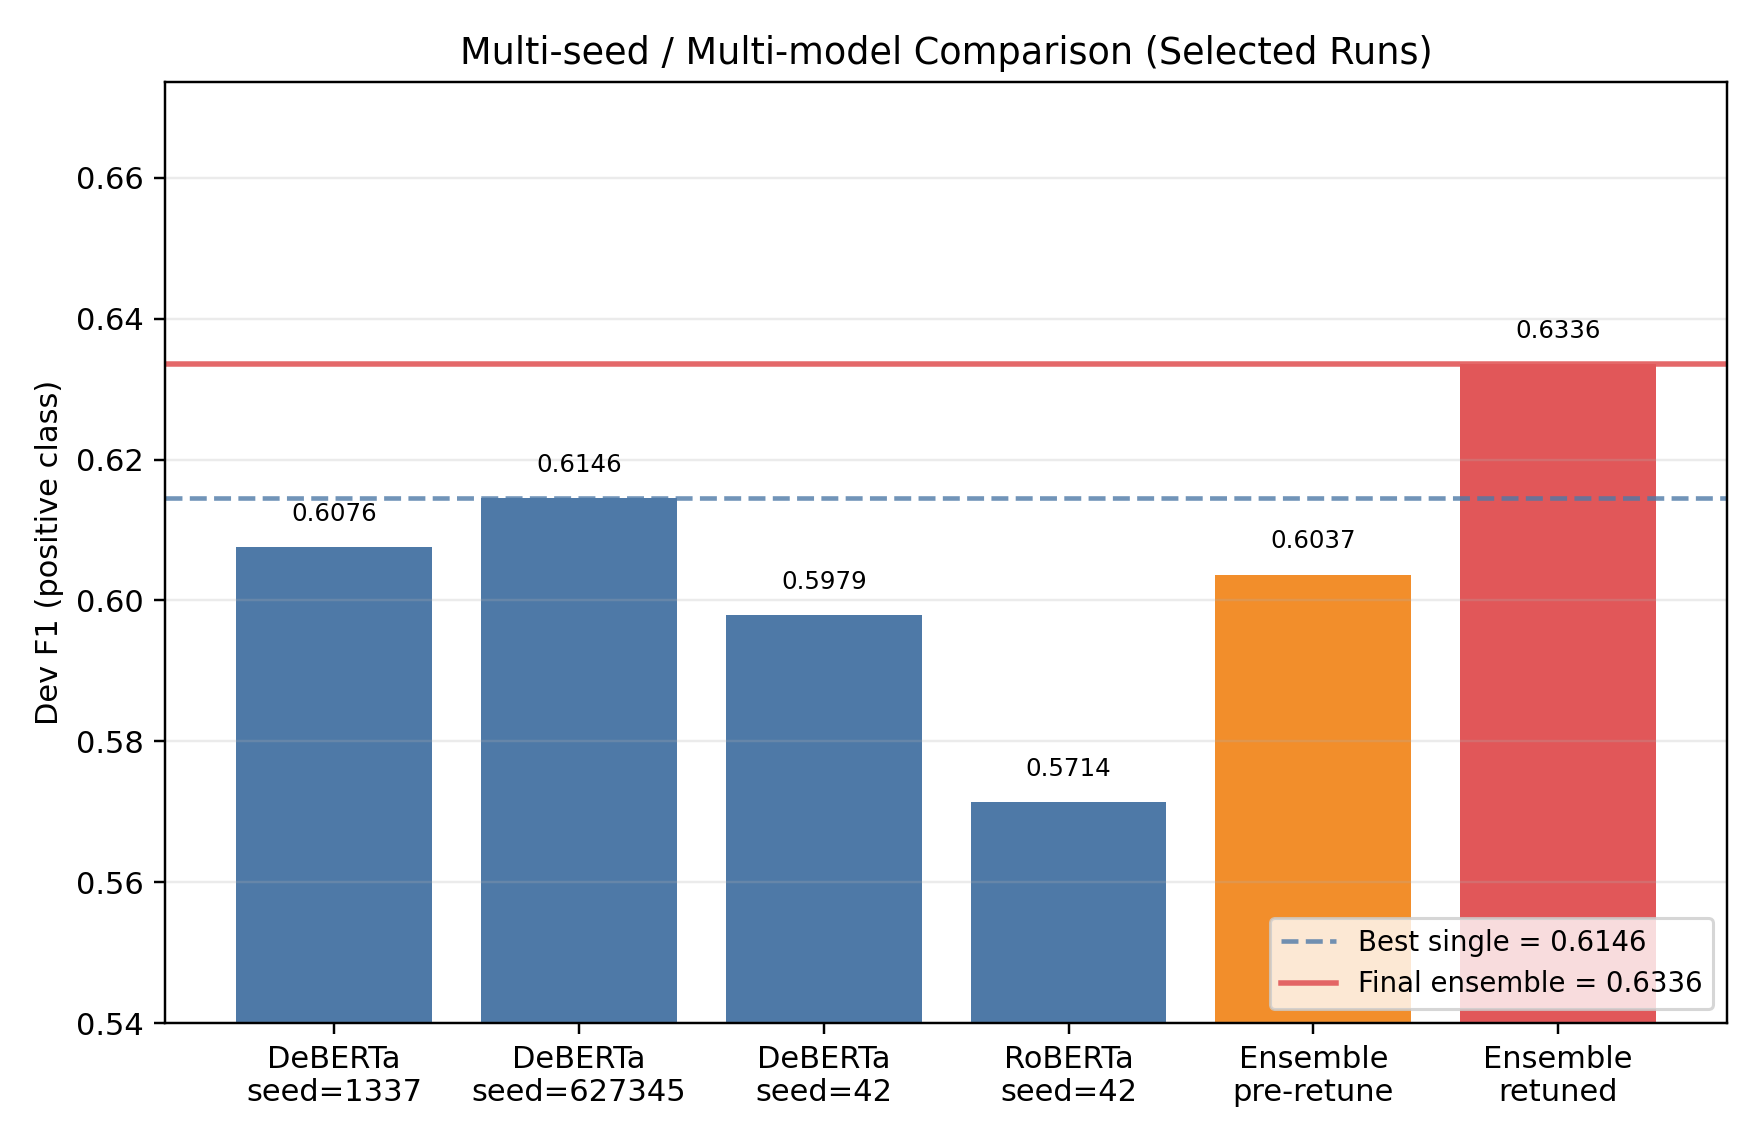
\includegraphics[width=0.74\linewidth]{figures/error_multiseed_comparison_dev.png}
  \caption{Multi-seed comparison for the selected runs and ensemble variants on dev. The final retuned ensemble outperforms every single run, showing the value of aggregation plus threshold recalibration.}
  \label{fig:error_multiseed_comparison_dev}
\end{figure}

\textbf{Interpretation of Figure \ref{fig:error_multiseed_comparison_dev}:}
The strongest single run reaches \(0.6146\) F1, while the final retuned ensemble reaches \(0.6336\), showing that ensembling plus threshold recalibration improves over all individual checkpoints rather than only matching the best seed.

\textbf{What the overall error profile shows:}
Across all views (confusion matrix, metric dashboard, PR curve, and seed comparison), the model is clearly above baseline and robust across runs, but its main residual limitation is still under-detection of subtle or implicit PCL cues.

\textbf{Baseline vs final overlap analysis:}
To make the improvement over baseline concrete at sample level, we compared baseline RoBERTa dev predictions against final ensemble dev predictions and grouped every dev example into four mutually exclusive cases: both models correct, both models incorrect, final-only correct, and baseline-only correct.
\begin{table}[H]
  \centering
  \small
  \begin{tabular}{lcc}
    \toprule
    Case (dev, \(n=2094\)) & Count & Share \\
    \midrule
    Both models correct & 1772 & 84.62\% \\
    Both models incorrect & 119 & 5.68\% \\
    Final model correct, baseline incorrect & 167 & 7.98\% \\
    Baseline correct, final model incorrect & 36 & 1.72\% \\
    \bottomrule
  \end{tabular}
  \caption{Direct overlap analysis between baseline and final-system correctness on official dev.}
  \label{tab:baseline_final_overlap_dev}
\end{table}

\textbf{Interpretation of Table \ref{tab:baseline_final_overlap_dev}:}
The final system changes 203 decisions relative to baseline (\(9.69\%\) of dev), and most of those changes are beneficial: 167 fixes versus 36 regressions (82.3\% beneficial among changed decisions), for a net gain of 131 correctly classified examples. The metric-level shift is consistent with this pattern: baseline TP/FP/FN \(=\) 139/226/60 (F1 \(=0.4929\)), whereas final TP/FP/FN \(=\) 134/90/65 (F1 \(=0.6336\)). In other words, the final system gives up a small amount of recall (\(-5\) TP) to remove a large number of false alarms (\(-136\) FP), which is exactly the trade-off that lifts positive-class F1.

\begin{table}[H]
  \centering
  \scriptsize
  \begin{tabularx}{\linewidth}{>{\raggedright\arraybackslash}X c >{\raggedright\arraybackslash}X}
    \toprule
    Error concentration on dev & Count & Interpretation \\
    \midrule
    FP in \texttt{homeless}/\texttt{in-need}/\texttt{poor-families}/\texttt{hopeless} & 65/90 (72.2\%) & Hardship/help vocabulary is often treated as a PCL trigger even in neutral reporting or service-delivery contexts. \\
    FN in \texttt{poor-families}/\texttt{homeless}/\texttt{women} & 37/65 (56.9\%) & Implicit condescension in these topics is frequently under-detected. \\
    Single-category positives in all positives & 50/199 (25.1\%) & These account for 22/65 FNs (33.8\%), suggesting one-cue positives are harder than multi-cue positives. \\
    \bottomrule
  \end{tabularx}
  \caption{Where the majority of remaining errors are concentrated.}
  \label{tab:error_concentration_dev}
\end{table}

\begin{table}[H]
  \centering
  \small
  \begin{tabular}{lcc}
    \toprule
    PCL category & Positives containing category & FN rate \\
    \midrule
    Authority\_voice & 38 & 36.8\% \\
    Poorer\_the\_merrier & 11 & 36.4\% \\
    Shallow\_solution & 36 & 36.1\% \\
    \bottomrule
  \end{tabular}
  \caption{Hardest category families on dev (highest false-negative rates).}
  \label{tab:error_category_fn}
\end{table}

\textbf{Manual inspection of failed samples:}
\begin{itemize}
  \item \textbf{False positives from humanitarian/action framing:} \texttt{par\_id 8453} (``helping Veterans in need''), \texttt{par\_id 8616} (``poor families ... save enough''), and \texttt{par\_id 8560} (``those left homeless receive shelter'') are predicted as PCL although they are largely informational/supportive. The model overfires on compassion/help tokens.
  \item \textbf{False negatives from implicit stereotyping or presupposition:} \texttt{par\_id 773} (``immigrant's job ... too dirty, too cold, too lonely'') and \texttt{par\_id 2001} (``not all ... come from poor families'') contain condescending assumptions but lack the strongest overt lexical cues, so the model predicts No PCL.
  \item \textbf{Category-specific misses consistent with dataset difficulty:} categories that require stronger pragmatic/world-knowledge interpretation (especially Authority voice and related implicit categories) remain harder, matching the higher FN rates above and the difficulty pattern reported in the original PCL paper.
  \item \textbf{Length effect is present but secondary:} FN examples are longer on average than FP examples (51.8 vs 48.4 tokens). This is consistent with our EDA observation that subtle positive cues can be distributed across longer contexts, but the larger issue is still semantic ambiguity rather than pure sequence length.
\end{itemize}

\textbf{Error-analysis insight for model development:}
The remaining errors are not random. They cluster around (i) lexical trigger overfiring in non-condescending aid narratives and (ii) under-detection of implicit, one-cue condescension. This explains why thresholding and class balancing helped, but also why further gains likely require better contextual disambiguation (especially for authority-style and other implicit PCL cues) rather than only more aggressive threshold shifts.

\subsubsection{Ablation study (2.5 marks):}

\textbf{Objective:}
This ablation study tests which components of the final system are genuinely responsible for the dev-set gains. The goal is to isolate causal contribution by changing one component at a time while keeping the rest of the pipeline fixed.

\newpage
\textbf{Protocol (step-by-step):}
\begin{enumerate}[leftmargin=*]
  \item \textbf{Reference system definition:} the control setup is the same 4-epoch system used for final reporting (three DeBERTa-v3 seeds + one RoBERTa-base seed, weighted soft-voting, tuned dev threshold).
  \item \textbf{Controlled variants:} we ablated one component per run: (i) remove weighted sampler, (ii) force fixed threshold 0.50, (iii) reduce max sequence length to 128, (iv) disable text cleanup.
  \item \textbf{Training/inference consistency:} each variant keeps the same selected model identities, optimizer family, and ensemble construction procedure, so the changed component is the only intended difference.
  \item \textbf{Single-model scoring:} for each variant, we report the best single-model dev F1 among the four members.
  \item \textbf{Ensemble scoring:} we then aggregate the four members using weighted soft-voting and report precision, recall, F1, and the decision threshold used for that variant.
  \item \textbf{Comparison target:} all deltas are computed against the 4-epoch control system to keep the analysis consistent with the rest of the report.
\end{enumerate}

\begin{table}[H]
  \centering
  \small
  \resizebox{\linewidth}{!}{%
  \begin{tabular}{lrrrrrr}
    \toprule
    Variant & Best single F1 & Ensemble P & Ensemble R & Ensemble F1 & $\Delta$ single & $\Delta$ ensemble \\
    \midrule
    Control & 0.6146 & 0.5982 & 0.6734 & 0.6336 & ref & ref \\
    No weighted sampler & 0.5940 & 0.6146 & 0.6031 & 0.6056 & -0.0206 & -0.0280 \\
    Fixed threshold (0.50) & 0.5953 & 0.5375 & 0.6960 & 0.6034 & -0.0193 & -0.0302 \\
    Max length = 128 & 0.6089 & 0.5753 & 0.6684 & 0.6182 & -0.0057 & -0.0154 \\
    No text cleanup & 0.6034 & 0.5885 & 0.6508 & 0.6180 & -0.0112 & -0.0156 \\
    \bottomrule
  \end{tabular}
  }
  \caption{Task 1 ablation summary under the 4-epoch study setting. Deltas are relative to the control row.}
  \label{tab:ablation_task1}
\end{table}

\textbf{Results and interpretation:}
Two ablations clearly dominate the performance drop:
\begin{itemize}
  \item \textbf{No weighted sampler} lowers ensemble F1 from 0.6336 to 0.6056 (\(-0.0280\)). Precision rises to 0.6146 but recall drops to 0.6031, showing that without imbalance-aware sampling the system becomes conservative and misses too many positive PCL cases.
  \item \textbf{Fixed threshold 0.50} lowers ensemble F1 to 0.6034 (\(-0.0302\)), the largest degradation. Recall increases (0.6960) but precision drops to 0.5375, confirming that threshold calibration is not optional in this imbalanced setting.
\end{itemize}

The other two ablations are meaningfully smaller:
\begin{itemize}
  \item \textbf{Max length 128} gives F1 \(=0.6182\) (\(-0.0154\)), indicating that truncating context hurts but does not collapse the model.
  \item \textbf{No text cleanup} gives F1 \(=0.6180\) (\(-0.0156\)), showing preprocessing contributes, but less than sampling and calibration.
\end{itemize}

\textbf{What this lets us infer about the model:}
\begin{itemize}
  \item The largest share of the final performance gain comes from \textbf{decision calibration and class-imbalance handling}, not from a single architecture choice alone.
  \item \textbf{Sequence budget and cleanup are second-order gains}: they improve robustness and consistency, but they are not the primary drivers of F1.
  \item The ensemble is strongest when members are both reasonably calibrated and class-balanced; when these properties are weakened, ensemble aggregation cannot recover the lost signal.
\end{itemize}

Overall, the ablation evidence supports the final system design: weighted sampling + tuned threshold are the highest-impact pieces, while length and cleanup provide additional but smaller gains.
\section{Conclusion and Future Work:}
\textbf{What we set out to do and what we built:}
We approached this coursework as a full NLP research cycle for imbalanced binary PCL detection. We started by critically reviewing the task paper, then used EDA to identify actionable properties of the data: severe class imbalance and a non-trivial long-tail of paragraph lengths. Based on those findings, we designed a system around two principles: robust positive-class recovery and stable decision calibration. Concretely, we trained multiple transformer runs (DeBERTa-v3 and RoBERTa-base across seeds), selected strong members through a controlled internal validation protocol, and combined them with a weighted soft-vote ensemble plus threshold tuning on the official dev set.

\textbf{What we achieved:}
Our final dev result is positive-class F1 \(=0.6336\), improving over the coursework baseline of \(0.4800\) by \(+0.1536\) absolute (\(+32.0\%\) relative). This gain came from repeated seed-level performance and ensemble aggregation that improved the overall precision--recall balance. In practical terms, we achieved a substantially stronger detector while preserving the required submission format and official ordering constraints for \texttt{dev.txt} and \texttt{test.txt}.

\textbf{What we learned from error analysis and ablation:}
Our local evaluation showed a consistent residual error pattern: false positives are concentrated in humanitarian/help framing where compassionate wording is not necessarily condescending, while false negatives often involve implicit or subtle condescension that lacks obvious lexical triggers. The ablation study reinforced this: class-imbalance handling and threshold calibration were the highest-impact components, while sequence length policy and cleanup steps provided smaller but still meaningful gains. Together, these findings explain both why the final system improves on baseline and where the remaining performance ceiling comes from.

\textbf{Limitations and future work:}
Because official test labels are hidden, detailed diagnostics are dev-based, and dev-tuned thresholds may be mildly optimistic. In a follow-up iteration, we would (i) add stronger calibration protocols that reduce dependence on a single dev threshold, (ii) integrate span/category supervision to better capture implicit PCL cues, (iii) apply targeted augmentation or contrastive training to reduce lexical-trigger overfiring, and (iv) report uncertainty and statistical significance across seeds more explicitly. Overall, this project shows that we can move from baseline reproduction to a defensible, evidence-driven model improvement pipeline, while making clear what remains unresolved and how we would address it next.
\newpage
\begin{thebibliography}{9}
  \bibitem[Perez-Almendros et~al.(2020)Perez-Almendros, Espinosa-Anke and Schockaert]{perez2020}
  Perez-Almendros, C., Espinosa-Anke, L. and Schockaert, S. (2020) `Don't Patronize Me! An Annotated Dataset with Patronizing and Condescending Language towards Vulnerable Communities', in \textit{Proceedings of the 28th International Conference on Computational Linguistics}. Barcelona, Spain (Online), 8--13 December. pp. 5891--5902. Available at: \url{https://aclanthology.org/2020.coling-main.518/} (Accessed: 18 February 2026).

  \bibitem[Liu et~al.(2019)Liu, Ott, Goyal, Du, Joshi, Chen, Levy, Lewis, Zettlemoyer and Stoyanov]{liu2019roberta}
  Liu, Y. \textit{et al.} (2019) `RoBERTa: A Robustly Optimized BERT Pretraining Approach'. Available at: \url{https://arxiv.org/abs/1907.11692} (Accessed: 4 March 2026).

  \bibitem[He et~al.(2021)He, Gao and Chen]{he2021debertav3}
  He, P., Gao, J. and Chen, W. (2021) `DeBERTaV3: Improving DeBERTa using ELECTRA-Style Pre-Training with Gradient-Disentangled Embedding Sharing'. Available at: \url{https://arxiv.org/abs/2111.09543} (Accessed: 4 March 2026).

  \bibitem[Koleczek et~al.(2022)Koleczek, Scarlatos, Pereira and Karkare]{koleczek2022umass}
  Koleczek, D., Scarlatos, A., Pereira, P.L. and Karkare, S.M. (2022) `UMass PCL at SemEval-2022 Task 4: Pre-trained Language Model Ensembles for Detecting Patronizing and Condescending Language', in \textit{Proceedings of the 16th International Workshop on Semantic Evaluation (SemEval-2022)}. Seattle, United States, pp. 445--453. Available at: \url{https://aclanthology.org/2022.semeval-1.60/} (Accessed: 4 March 2026).
\end{thebibliography}
\end{document}
